\documentclass[aps,pra,reprint,onecolumn,10pt,notitlepage,nofootinbib]{revtex4-2}
\usepackage{amsmath,amssymb,graphicx,booktabs,array}
\usepackage[T1]{fontenc}
\usepackage{xurl}
\usepackage[colorlinks=true,linkcolor=blue,citecolor=blue,urlcolor=blue]{hyperref}
\newcolumntype{L}[1]{>{\raggedright\arraybackslash}p{#1}}
\emergencystretch=2em
\pdfstringdefDisableCommands{\def\\{ }}
\hypersetup{pdftitle={VigilODE RVJ/NAG theory and bounded native validation},pdfauthor={VigilODE research and validation record}}
\begin{document}
\title{Original-equation certification and quotient observables in VigilODE:\\
theory-first integration of the RVJ/NAG research and a bounded native validation}
\author{VigilODE research and validation record}
\noaffiliation
\date{October 28, 2026}
\begin{abstract}
We critically integrate the latest cumulative VigilODE validation, the supplied
RVJ/NAG research archive, and conditional earlier polyalgorithm results.
Three independent theoretical tasks precede parent admission and three coding
tasks. For a fixed cyclic algebraic closure we prove sharp Bernstein weights
$3/4$ and $25/32$, a safe exponential-free physical-error recurrence, and an
endpoint reuse identity. A scalar $O(n)$ lift avoids runtime Jacobian assembly,
matrix factorization, Newton iteration and derivative callbacks. For an explicit
quartic quotient, a multiplicity-preserving trace remains defined through a
triple root and admits a shared polynomial field; its semantics cannot replace
a selected physical root. The published execution source passes 15 native unit
tests, 732,947 independent exact-rational checks covering every exported slab,
and 10 supporting symbolic identities. At the same exact whole-state error cap
$10^{-8}$, the first passing registered cyclic grid changes from 64 to 32 steps;
native whole-call median speed ratios are 8.72--9.33 in the measured cohort.
Trace field kernels improve, but the complete candidate-trajectory measurements
are mixed and do not establish a speedup. We retain rejected grids, inherited
negative results, unresolved singular-branch and multivariate-quotient questions,
and all cumulative qualification gates. The general production status is HOLD.
\end{abstract}
\maketitle

\section{Scope, evidence and the latest-PR audit}

The execution source is
\begin{center}\small\path{64004e23042f2cf076da5378be724f50c3856f4c}.\end{center}
It was published and remotely read back before the scientific run. Its source
tree is \path{67564b455011252fdc1fb811c09baeea9f2bd31f}.
The parent is PR96, commit
\path{13f3298bd0213f121e07385903f9508c435ad6a1}.
PR95, commit \path{36104bfc65d1fdc695c8acea383c54b50a1c4e78},
was read as a separate theoretical input and was not merged.
The delivery branch is \path{research/production-rvj-nag-20261028}.
The supplied JSON and ZIP, and 23 byte-preserved selected source files, are
bound by the intake manifest. Historical measurements are inputs to criticism;
they are not the baseline for cross-host or cross-language speed ratios.

PR96 contains useful scoped repairs: an exact-rational squared residual check
for the returned Givens solution and a corrupted-answer control, explicit
entered/refused/completed/failed callback accounting, and focused lint evidence.
We verified 24 compact evidence hashes and five selected source hashes.
The measured-to-final PR96 code difference in the relevant runtime/tool paths
is empty. These facts do not complete its remaining production gates.
The prior authority check had 49 unresolved references, Q-API remained HOLD,
the six N tasks were unfinished, and all ten interaction gates were NOT\_RUN.
The W-filtered negative cost ratio $15/7$ exceeded the declared $1.3$ threshold;
the inaccurate Off result is retained. An earlier timeout and its extended
test run overlap and must not be added as independent test counts.

Some older raw files and an exact Givens receipt were left in unavailable
temporary directories; compact summaries are not fresh replays. PR96 also
distinguished its preregistration commit from a later actual execution source
that had not been remotely published before execution. The present cohort
closes that provenance gap for its own source only. Existing formatting,
ignored-feature, vendor, public-API and external-client obligations remain.
The final unmodified authority check first timed out during lazy object
retrieval. A cached-object run with lazy fetch disabled failed with 178
distinct unallowlisted missing objects and 919 failure citations. This
partial-clone result is not directly comparable with the earlier fuller-checkout
count of 49; missing objects can include blobs. Three new-node citations refer
to the byte-preserved external BASS commit/blob input, which the untyped
repository checker treats as VigilODE authority. No allowlist was expanded.
The complete audit and cumulative correction counters are delivered separately
in \path{theory/PR96_AUDIT.md}, \path{theory/PRODUCTION_GATES.json}, and
\path{LOCAL_DEVELOPMENT_PLAN.json}.

\subsection{Research order and admissible claims}

The theoretical agents investigated (i) original-equation cyclic certificates,
(ii) trace algebra and branch semantics, and (iii) PR96 evidence and applicability.
The parent reviewed those results and issued a bounded theory admission before
runtime implementation. The coding phase separated the two native modules
from the independent exact oracle, followed by an adversarial review.
One coherent prepublication correction episode is charged to inherited N03
and N05, each now $1/3$. There were no postpublication native repairs.
R-STRUCT and R-ADAPT remain exhausted at $3/3$; Q-LEDGER remains $1/3$.

The public modules are opt-in structured components, rather than a completed
generic stiff solver. A polyalgorithm may choose between certified candidates
only after their original model, requested observable, physical norm, clock,
checkpoint and output schedule agree. The cyclic small-real branch and the
all-complex multiplicity trace are different targets. A shared cost model is
meaningful only within a common admissible target.

% Theory fragment for the parent REVTeX report. No standalone preamble.
% Derivations: theory/CLOSURE.md and theory/TRACE.md.
% Bibliography keys are supplied by the parent: MRD2018, BFSS2002, CLM2025.

\section{Original-equation certificates for the cyclic closure}
\label{sec:cyclic-theory}

The cyclic problem has indices modulo $n$ and original equations
\begin{align}
 G_i(x,q)&=q_i+\frac14q_{i+1}^{2}-x_i=0,\label{eq:cyclic-original}\\
 \dot x_i=f_i(x,q)&=-x_i+\frac{q_i+q_{i+1}}{16}+c_i,
 \qquad c_i=\frac1{32}+\frac{i\bmod3}{256}.
\end{align}
The declared branch starts at $x=q=0$, with physical time $0\le t\le1$,
and domains $X=[-1/8,1/8]^n$, $Q=[-1/4,1/4]^n$.
The native specialization admits $n=4,8,16$.
The required error is the supremum over the entire time interval and all
slow and algebraic coordinates, in the original infinity norm, with cap
$10^{-8}=1/100000000$.

\paragraph{Proposition C1: branch and physical-error transfer.}
There is a unique $q(x)\in Q$ for each $x\in X$. Moreover,
\begin{align}
 \|q(x)-q(z)\|_\infty&\le\frac87\|x-z\|_\infty,\label{eq:cyclic-rootlip}\\
 \|\widehat q-q(x)\|_\infty&\le\frac87\|G(x,\widehat q)\|_\infty
 \quad(\widehat q\in Q).
\end{align}
The reduced field $F(x)=f(x,q(x))$ contracts at rate $\lambda=6/7$.

\emph{Proof.}
The map $T_x(q)_i=x_i-q_{i+1}^2/4$ maps $Q$ into
$[-9/64,1/8]^n\subset Q$ and contracts with factor $1/8$.
Subtracting its fixed-point equations, or comparing $\widehat q$ to its
fixed point, gives the two bounds. On an upper face of $X$, $f_i\le-7/128$;
on a lower face, $f_i\ge1/8$. Thus the exact slow solution stays in $X$.
Writing $F=-x+Cq+c$ with $\|C\|_\infty=1/8$ gives the maximum-coordinate
Dini contraction rate $1-(1/8)(8/7)=6/7$.

For a differentiable candidate $(\widehat X,\widehat Q)$ in $X\times Q$,
define the original residuals
\begin{equation}
 R_f=\widehat X'-f(\widehat X,\widehat Q),\qquad
 R_g=G(\widehat X,\widehat Q).
\end{equation}
Whole-slab bounds $\|R_f\|_\infty\le D_f$ and
$\|R_g\|_\infty\le D_g$, with
$e=\|\widehat X-x_{\rm exact}\|_\infty$, imply
\begin{align}
 D^+e&\le-\lambda e+\delta,
 \qquad\delta=D_f+D_g/7,\label{eq:cyclic-error-ode}\\
 \|\widehat Q-q(x_{\rm exact})\|_\infty
 &\le\frac87(e+D_g).
\end{align}
This comparison uses a residual evaluated on the numerical reconstruction.
It therefore retains the exact-flow error anchor; an exact-input-only
discrete truncation estimate cannot be substituted without a separate
stability argument. Adjoint DAE analysis for linear quantities of interest
provides complementary output contracts~\cite{CLM2025}; the present contract
retains every physical coordinate throughout the path.

\subsection{Finite lift and the exact reconstructed path}

Let $b_i=q_{i+1}/2$, $(Av)_i=b_i v_{i+1}$ and $P=\prod_i b_i$.
Then $A^n=PI$ and
\begin{equation}
 (I+A)\sum_{k=0}^{n-1}(-A)^k=[1-(-1)^nP]I.
\end{equation}
The denominator $d=1-(-1)^nP$ satisfies $d\ge1-8^{-n}>0$ on $Q$.
Solving $v_i=f_i-b_i v_{i+1}$ by composition around the cycle and a backward
substitution computes the inverse action in $O(n)$ scalar operations.
For the exact rational lift $s(y)=(f,v)$, $y=(x,q)$,
\begin{equation}
 G_qv=f                                                        \label{eq:cyclic-tangency}
\end{equation}
holds even at endpoints with $G\ne0$.
The native circuit evaluates this declared analytic structure without a
Jacobian, JVP, AD or Newton callback. The identity is specific to these
equations and is not a black-box result for arbitrary closures.

Stored finite binary64 endpoints $y_0,y_1$ denote exact dyadics.
The certified Hermite polynomial uses the \emph{exact rational} slopes
$s_j=s(y_j)$, enclosed numerically by outward arithmetic. With
$B_j^m(\theta)=\binom mj\theta^j(1-\theta)^{m-j}$,
its cubic Bernstein controls are
\begin{equation}
 Y_0=y_0,\quad Y_1=y_0+hs_0/3,\quad
 Y_2=y_1-hs_1/3,\quad Y_3=y_1.                              \label{eq:cyclic-controls}
\end{equation}
The componentwise control hull must lie in $X\times Q$.
The Bernstein convex-hull property provides the whole-interval range
enclosure~\cite{MRD2018}. Arithmetic enclosure remains necessary: rounded
endpoint slopes would define a different path. The supplied dense-query
interface returns an interval enclosure of the declared path.

\paragraph{Proposition C2: sharp slow-residual weight.}
For one slow component let $X_j$ denote its controls and set
\begin{align}
 D_0&=f_i(y_0),\qquad D_2=f_i(y_1),\\
 D_1&=3(X_2-X_1)/h,\\
 r_1&=D_0/3+2D_1/3-f_i(Y_1),\\
 r_2&=2D_1/3+D_2/3-f_i(Y_2).
\end{align}
The cubic Bernstein residual coefficients are exactly $(0,r_1,r_2,0)$,
and consequently
\begin{equation}
 D_f\le\frac34\max_i\{|r_{1,i}|,|r_{2,i}|\}.               \label{eq:cyclic-df}
\end{equation}
\emph{Proof.}
Degree elevation of the quadratic derivative gives the displayed interior
coefficients. Affineness of $f$ gives field controls $f(Y_j)$; the endpoint
differences vanish by the exact-slope definition. The residual equals
$3\theta(1-\theta)[(1-\theta)r_1+\theta r_2]$.
Since $3\theta(1-\theta)\le3/4$, Eq.~\eqref{eq:cyclic-df} follows, with
equality possible for equal, same-signed $r_1,r_2$ at $\theta=1/2$.

\paragraph{Proposition C3: three interior algebraic coefficients.}
For component $i$ set $d_j=Q_{i,j}-X_{i,j}$, $z_j=Q_{i+1,j}$ and
$g_\ell=G_i(y_\ell)$. The degree-six residual coefficients are
\begin{equation}
 (g_0,g_0,\beta_2,\beta_3,\beta_4,g_1,g_1),\qquad
 \beta_k=E_k+S_k/4,                                      \label{eq:cyclic-gcoeff}
\end{equation}
where the exact rational expressions are
\begin{align}
 E_2&=(d_0+3d_1+d_2)/5,&S_2&=(2z_0z_2+3z_1^2)/5,\\
 E_3&=(d_0+9d_1+9d_2+d_3)/20,&
 S_3&=(z_0z_3+9z_1z_2)/10,\\
 E_4&=(d_1+3d_2+d_3)/5,&S_4&=(2z_1z_3+3z_2^2)/5.
\end{align}
\emph{Proof.}
Cubic-to-degree-six elevation gives $E_k$ and the Bernstein product rule
gives $S_k$. Equation~\eqref{eq:cyclic-tangency} makes the two endpoint
derivatives of $G(Y(\theta))$ zero. The derivative formulas
$6(\beta_1-\beta_0)$ and $6(\beta_6-\beta_5)$ then give the repeated
endpoint coefficients, without assuming exact constraint satisfaction.

Let $g$ bound the endpoint magnitudes and $m$ the three interior magnitudes,
over all components. The interior basis weight is
\begin{equation}
 w=B_2^6+B_3^6+B_4^6=15u^2-10u^3,
 \qquad u=\theta(1-\theta)\in[0,1/4].
\end{equation}
It increases with $u$ and attains $25/32$. Hence
\begin{equation}
 D_g\le\max\{g,(7g+25m)/32\}.                             \label{eq:cyclic-dg}
\end{equation}
The weight is sharp for this coefficient-information class. All these
constants follow from exact polynomial identities; none is fitted.

\paragraph{Proposition C4: endpoint reuse.}
The same represented endpoint and model/arithmetic identity define the
same exact slope and original residual. Thus $N$ consecutive slabs need
$N+1$ endpoint preparations instead of $2N$.
The native reuse check requires every endpoint bit, dimension and model
epoch to agree; branch, domain and arithmetic provider are fixed by the
module. For a nonautonomous extension the physical time would also belong
to this identity. A streaming consumer needs only the adjacent prepared
endpoints. This is an exact work reduction, with runtime effects measured
separately.

\subsection{A safe exponential-free error recurrence}

\paragraph{Proposition C5: maximum of two rational envelopes.}
Let $E,\delta,h\ge0$, $\lambda>0$ and $z=\lambda h$. Define
\begin{align}
 U_1&=\frac{E+h\delta}{1+z},&
 U_2&=\frac{(1-z/2)E+h\delta}{1+z/2},\\
 E_+&=\max(U_1,U_2),&E_{\rm whole}&=\max(E,E_+).            \label{eq:cyclic-rational-radius}
\end{align}
These enclose the endpoint and whole-slab comparison solution of
Eq.~\eqref{eq:cyclic-error-ode}.

\emph{Proof.}
Writing $w=\delta/\lambda$, the exact comparison is
$T(h)=w+(E-w)e^{-z}$. For $z\ge0$,
\begin{equation}
 \frac{1-z/2}{1+z/2}\le e^{-z}\le\frac1{1+z}.
\end{equation}
The upper inequality follows from $e^z\ge1+z$. For $0\le z<2$ the lower
one follows by integrating
$[\log((1+z/2)/(1-z/2))]'=1/(1-z^2/4)\ge1$; for $z\ge2$ its left side
is nonpositive. Use the upper exponential bound if $E\ge w$ and the lower
one if $E\le w$. The identity
\begin{equation}
 U_1-U_2=\frac{hz(\lambda E-\delta)}{2(1+z)(1+z/2)}
\end{equation}
shows that the maximum selects the safe expression. The scalar comparison
is monotone within the slab, yielding the whole-slab maximum.
In particular $U_1$ alone is invalid at $E=0$, $\delta>0$, $h>0$.

The independently valid inherited alternative is
$E_+=E/(1+\lambda h)+h\delta$, $E_{\rm whole}=E+h\delta$.
The two recipes are separate native comparison arms. The final algebraic
radius is $(8/7)(E_{\rm whole}+D_g)$. Rational constants, coefficients and
radius updates are evaluated outward under the core arithmetic assumptions;
nonfinite inputs and failed arithmetic are refused. The dyadic physical
clock has no uncharged time-label displacement. Admission compares with
the exact rational cap, rather than enlarging it by binary64 rounding.

\section{Typed quotient observables through a discriminant}
\label{sec:trace-theory}

\paragraph{Theorem T1: fixed rank with multiplicity.}
For a monic degree-$d$ polynomial $P$ and a polynomial observable $h$,
the multiplication operator on $\mathcal A=\mathbb C[z]/(P)$ satisfies
\begin{equation}
 \operatorname{Tr}_{\mathcal A}(m_h)
 =\sum_{r:P(r)=0}m_r h(r),\qquad \sum_r m_r=d.              \label{eq:trace-multiplicity}
\end{equation}
No square-free condition is needed. Monic division gives a fixed free basis
$1,z,\ldots,z^{d-1}$ even before parameter specialization. In the local
factor $\mathbb C[z]/((z-r)^{m_r})$, multiplication by $h$ is triangular
with diagonal $h(r)$ in the basis of powers of $z-r$. Its trace is
$m_rh(r)$; summing local factors proves the formula. If the coefficients of $P$ and $h$ depend polynomially on the parameters,
polynomial parameter dependence follows directly from monic reduction. This is the classical
trace/power-sum relation~\cite{BFSS2002}, specialized here with explicit
query semantics and finite-arithmetic obligations.

For the original two-equation family
$q_1^2+q_2=a$, $q_2^2+q_1=b$, elimination without division gives
\begin{equation}
 P_{a,b}(z)=z^4-2az^2+z+a^2-b,
 \qquad q_1=z,\quad q_2=a-z^2.                            \label{eq:trace-quartic}
\end{equation}
The quotient is therefore free of rank four at every $(a,b)$.
Its power sums are
\begin{align}
 &(S_0,S_1,S_2,S_3)=(4,0,4a,-3),\\
 &S_4=4a^2+4b,\quad S_5=-10a,\quad S_6=4a^3+12ab+3.
\end{align}
They follow from Newton identities, or directly by monic reduction and
Eq.~\eqref{eq:trace-multiplicity}. For $k>4$,
$S_k=2aS_{k-2}-S_{k-3}-(a^2-b)S_{k-4}$.
In particular $\operatorname{Tr}q_1=\operatorname{Tr}q_2=0$,
$\operatorname{Tr}(q_1q_2)=3$, and
$\operatorname{Tr}(q_1^2q_2^2)=4ab+3$.

At $a=b=3/4$,
\begin{equation}
 P=(z-1/2)^3(z+3/2),\qquad
 S_k=3(1/2)^k+(-3/2)^k.                                  \label{eq:trace-triple}
\end{equation}
The triple point contributes length three. Deduplicating roots changes
$S_0$ from $4$ to $2$ and $S_1$ from $0$ to $-1$.
The accepted query explicitly requests all complex roots with algebraic
multiplicity. A selected real branch is a different target: at $(a,b)=(2,2)$
the regular branch $(q_1,q_2)=(1,1)$ has determinant $4q_1q_2-1=3$ and
$q_1=1$, whereas both $\operatorname{Tr}q_1$ and its average are zero.
Thus a trace cannot be substituted as that branch's velocity, even away
from a singularity. The native interface also refuses real-only semantics.

\subsection{Shared field and a proved physical contraction constant}

The declared aggregate field is
\begin{align}
 \mathcal F_1&=-a+S_2/32+S_4/128+S_6/512,\\
 \mathcal F_2&=-b+S_2/64+S_4/64+S_6/256.
\end{align}
Exact substitution yields a single shared nonlinear circuit,
\begin{align}
 N(a,b)&=\frac{4a^3+16a^2+12ab+16b+3}{512},\\
 \mathcal F_1&=-7a/8+N,&\mathcal F_2&=-b+a/16+2N.          \label{eq:trace-shared}
\end{align}
Consequently $\mathcal F_2-2\mathcal F_1=29a/16-b$.
An evaluation error $e_N$ in the shared circuit contributes exactly
$(e_N,2e_N)$ before surrounding-operation errors. Outward interval
evaluation encloses the original polynomial for the declared parameter
intervals and preserves the same query. No inverse root separation enters.

\paragraph{Proposition T3: sharp unweighted row-bound constant.}
On $D=[1/2,1]^2$, the off-diagonal field derivatives are nonnegative and the
diagonals negative. Their row sums increase with $a,b$. At $(1,1)$,
\begin{equation}
 D\mathcal F=
 \begin{pmatrix}-49/64&7/128\\9/32&-57/64\end{pmatrix}.
\end{equation}
The row sums are $-91/128$ and $-39/64$. Therefore
\begin{equation}
 \mu_\infty(D\mathcal F)\le-39/64.                        \label{eq:trace-rate}
\end{equation}
The constant is sharp for this row-sum proof on this domain, since the
second row attains equality. Differentiation supplies an offline proof of
the bound; the runtime field uses only the polynomial circuit.

The controlled original target used to cross the discriminant is
\begin{align}
 p(t)&=\frac34+\frac t8+\frac{t^5}{64},\qquad -1\le t\le1,\\
 \dot y&=\mathcal F(y)+p'(t)\mathbf1-\mathcal F(p(t)\mathbf1),\\
 y(-1)&=(39/64)\mathbf1.                                  \label{eq:trace-controlled}
\end{align}
Its exact solution is $y=p(t)\mathbf1$, with terminal value
$(57/64)\mathbf1$. Since $p'>0$ and
$\operatorname{disc}P_{a,a}=(4a-3)^3(4a+1)$, it crosses the triple-root
parameter at $t=0$. The time-only forcing preserves
Eq.~\eqref{eq:trace-rate}. A candidate's uniform original-field defect
$\delta$ and a certified domain tube then give
\begin{equation}
 e(t_i+s)\le e^{-(39/64)s}E+
 \frac{1-e^{-(39/64)s}}{39/64}\delta .                     \label{eq:trace-physical}
\end{equation}
A strict boundary margin with a whole-slab error bound closes the usual
first-exit argument when domain containment is not already known.
Trace arithmetic included in an original-field interval residual is charged
once. Endpoint agreement with $p(t)$ is an independent control and does not
replace the whole-path residual/tube obligation.

\section{Boundaries of the admitted mathematical scope}
\label{sec:theory-boundaries}

The selected-branch atlas and the multiplicity-preserving trace have
different mathematical targets. The two supplied primitive charts share
the determinant $4q_1q_2-1$; their transition formulas do not establish
regular selected-root continuation at determinant zero. The cyclic domain
instead has the strictly positive denominator proved above. Trace regularity
at Eq.~\eqref{eq:trace-triple} follows from its monic rank-four algebra and
does not resolve a selected singular branch.

The separate F5 global incidence counts also remain open. The original
$116/58$ ordered/unordered totals omit a horizontal contribution $4/2$.
The resulting $120/60$ remains conditional on completeness of the retained
charts and exclusions. A reviewed transversality stratum with
$D=4\eta^3p+27\eta^2q+27pq=0$ has local length three despite regular
carrier data, so reduced point counting alone cannot certify the quotient
rank. A future multivariate trace provider must supply its full ideal,
localizations, basis or finite-freeness proof, local lengths and quotient
semantics. These incomplete global counts do not affect the independent
rank-four proof for Eq.~\eqref{eq:trace-quartic}.

The native components instantiate the bounded contracts proved here;
their measured validation is reported separately. Whole-model physical
certification for a different application still requires its original
closure/ODE, selected observable, domain, physical clock and representation
errors. Generic stiff integration, singular-branch continuation, arbitrary
sparse quotients and wider floating-point environments retain independent
theoretical and implementation obligations. No generic production claim
follows solely from the fixed-model certificates.


\section{Native implementation and independent verification}

The cyclic module uses the existing outward arithmetic primitives. Prepared
endpoints own the represented bits, model epoch, interval slope, original
constraint residual and denominator enclosure. A dyadic grid carries the
physical slab clock; finite/domain/epoch/clock failures are explicit refusals.
The cap is exactly $1/100000000$: a floating-point display value is not allowed
to enlarge it. The final admission uses an upward-rounded product with
$100000000$ and compares with one. An interval dense query encloses the exact
field-slope Hermite path to which the proof applies.

The trace module has an explicit all-complex algebraic-multiplicity query.
Selected-real and real-only queries are refused. It revalidates public interval
fields and rejects nonfinite arithmetic. Constant and linear polynomial queries
do not compute unused high moments that might overflow; all supplied
coefficients are nevertheless validated. Caller-owned counters retain work
on failed requests. The shared-field and necessary-moment routes evaluate the
same original aggregate target, with the same time-dependent forcing charged
to both trajectory routes.

The benchmark scope includes the private-workspace destruction inside the
cyclic total timer, and structured failure diagnostics preserve partial work.
It excludes the later consumer lifetime of returned output. This distinction
prevents allocation cleanup or failed preparation from disappearing merely
because a fast phase has finished.

\subsection{Oracle independence and coverage}

The exact Python oracle constructs a finite $n$-term cyclic inverse action,
rather than copying the native affine recurrence. It reconstructs Hermite
polynomials in the POWER basis from exact dyadic endpoint values and rational
original-field slopes, forms the original slow and constraint residuals, and
then converts them to Bernstein form. It checks every exported coefficient
interval, original-model domain, clock, radius and cap decision. The trace
oracle independently uses exact companion-matrix traces, repeated-root
multiplicity controls, the original moment field, and exact polynomial
whole-slab residual and tube bounds.

\begin{table}[h]
\caption{Completed validation at the published execution source. The native
unit count is restricted to the two added modules.}
\begin{ruledtabular}
\begin{tabular}{L{0.56\linewidth}r}
Check & Completed result \\
\hline
Cyclic / trace native unit tests & 6 / 9 PASS \\
New ignored tests & 0 \\
Independent rational assertions & 732,947 PASS \\
Distinct cyclic slabs / arm--slab records & 720 / 2,160 \\
Cyclic coefficient intervals & 383,040 \\
Trace trajectories / slabs & 10 / 992 \\
Registered Wolfram supporting identities & 10 / 10 PASS
\end{tabular}
\end{ruledtabular}
\end{table}

A corrupted cyclic coefficient interval and a distinct-root count at the
triple point are rejected by negative controls. No sampled supremum is treated
as a proof. The Wolfram identities support exact algebra only; the raw response
and file digest are stored, and the analytical proofs and floating-point
validation remain separate. SciSpace and Exa provided discovery; the cited
primary texts were inspected directly. Inaccessible and irrelevant search
results were not used as evidence.

\section{Registered measurements and phase profiles}

The native run started at 10:37:24 UTC on October 28, 2026, after the source
readback at 10:37:20 UTC. Rust 1.94.1 used the locked/offline dependencies and
the measurement profile (optimization level 3, no LTO, 16 codegen units).
Builds, tests and benchmarks were serialized under a shared lock.
The host was Linux on an AMD EPYC 9V74 with nine allowed CPUs; no explicit
taskset pinning or frequency control was recorded. These are shared-container
phase wall times and source work counters, not hardware performance counters.

Each native timing cell has one separate warmup and seven retained measured
repetitions with rotating or alternating route order. No slow repetition was
removed. The representative statistic is the median; minimum and maximum
are retained in the machine analysis. A ratio is baseline median divided by
candidate median. Paired-repeat ratios are a distinct descriptive statistic.
These repetitions provide neither a statistical holdout nor a universal
hardware-performance guarantee. Phase medians need not sum to the total median.

\subsection{Cyclic: matched cap and fixed candidate comparisons}

All three arms use identical compiled RK4 endpoint bits at a given grid.
The historical arm uses generic power-polynomial residual construction,
convolution and Bernstein conversion with the valid legacy radius.
Direct/legacy changes the certification circuit and endpoint reuse while
retaining that radius. Direct/tight additionally uses Eq.~\eqref{eq:cyclic-rational-radius}.
All share the same outward arithmetic; the baseline was not padded with
unnecessary endpoint checks.

\begin{table}[h]
\caption{First passing registered grid at the exact whole-state, whole-path
cap $10^{-8}$. Times are whole-call medians in milliseconds. The headline
always uses the same Direct/tight arm.}
\begin{ruledtabular}
\begin{tabular}{rrrrr}
$n$ & Historical, $N=64$ & Direct/legacy, $N=32$ & Direct/tight, $N=32$ & Hist./tight \\
\hline
4 & 3.148950 & 0.369877 & 0.361093 & 8.7206 \\
8 & 5.880571 & 0.640684 & 0.630028 & 9.3338 \\
16 & 11.620309 & 1.232214 & 1.263291 & 9.1984
\end{tabular}
\end{ruledtabular}
\label{tab:closure-matched}
\end{table}

The whole-state bounds for Direct/tight at $N=32$ are approximately
$8.40591\times10^{-9}$, $8.40984\times10^{-9}$ and
$8.40978\times10^{-9}$ for $n=4,8,16$.
Historical $N=64$ bounds are approximately $1.42\times10^{-9}$.
Thus Table~\ref{tab:closure-matched} compares costs meeting the same requested
cap, not two trajectories with identical realized error. The first passing
grid belongs to the preregistered set $\{16,32,64,128\}$ and is not a proof
of a globally minimal step count. Of 36 cells, 24 pass and 12 refusals remain.
An upper bound failing to certify the cap does not prove an actual violation.

At fixed $N=64$, Direct/tight whole-call ratios are 4.2534, 4.6292 and
4.7859 for $n=4,8,16$. Direct/legacy ratios are 4.5295, 4.5019 and 4.8700.
This fixes the candidate path and isolates the joint circuit/reuse
optimization. The larger matched-cap ratios include the additional benefit
of a coarser admissible grid. Endpoint interval slope evaluations drop from
128 to 65, with 63 reused endpoints. At the matched cap they drop from
128 to 33, and candidate RHS calls drop from 256 to 128.

\begin{figure}[h]
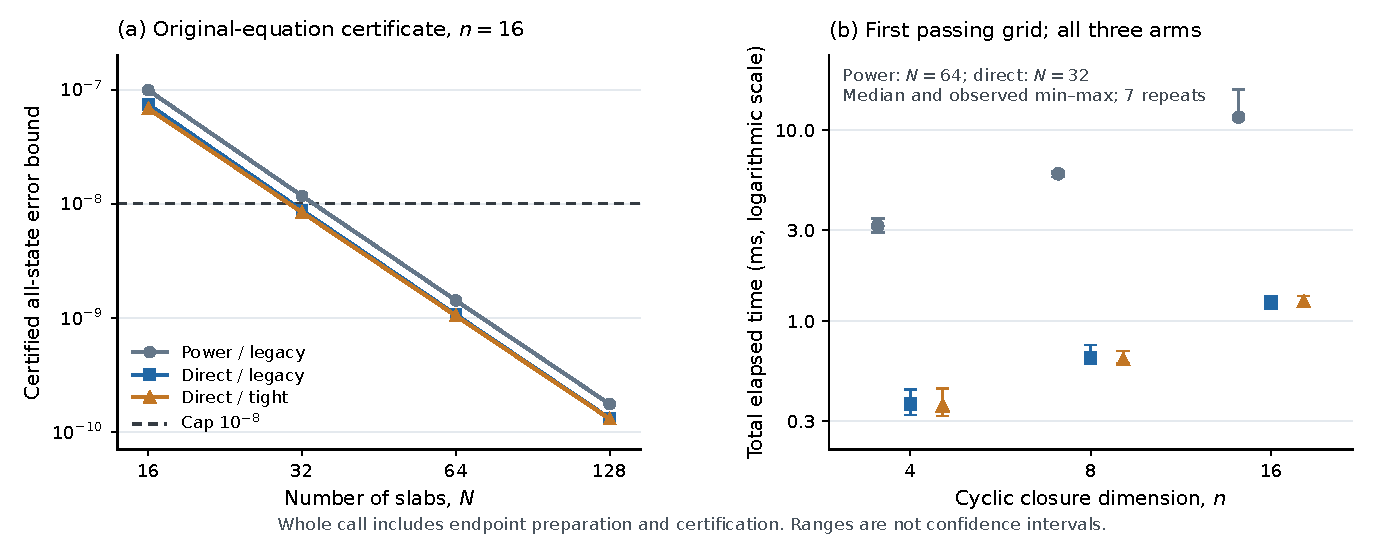
\includegraphics[width=\linewidth]{closure_results.pdf}
\caption{Cyclic evidence. Left: certified whole-state upper bounds at
$n=16$, not measured true errors. Right: first-passing total medians for all
three arms; bars span the retained minimum and maximum of seven repeats.
The old and new arms meet the same cap at different registered grids.}
\label{fig:closure}
\end{figure}

At $N=64$, preparation plus certificate accounts for 98.8--99.3\% of
historical total time and 95.4--97.0\% of Direct/tight time.
The dominant cost therefore remains certification. Direct paths eliminate
the generic convolution/transform calls, not every scalar multiplication.
The tighter radius decreases the bound but has the same first passing grid
as Direct/legacy. Several cells have a slower Direct/tight median with
overlapping ranges. It is not an independently established uniform speed
improvement. Candidate-only fluctuations do not show a new integrator gain,
because the candidate algorithm is unchanged.

\subsection{Trace: local savings and an adverse trajectory statistic}

Each field block contains 2,064 evaluations on the same retained inputs.
Each trajectory block contains 16 RK4 trajectories with $N=128$.
The necessary-moment field uses 13 scalar multiplications and 9 additions;
the shared field uses 8 and 7. These source arithmetic counters are not
measured processor FLOPs. Semantics/finite checks and actual field work are
charged; both trajectory routes include the same original forcing.

\begin{table}[h]
\caption{Trace blocks: seven-repeat medians, with retained min--max ranges
in microseconds. Values above one in the last column favor the shared route.}
\begin{ruledtabular}
\begin{tabular}{lrrr}
Phase & Direct median [min,max] & Shared median [min,max] & Direct/shared \\
\hline
Candidate field & 75.404 [74.502,165.469] & 63.145 [62.644,71.337] & 1.1941 \\
Interval field & 1143.962 [1050.851,1411.494] & 763.960 [677.179,1039.664] & 1.4974 \\
Combined field & 1184.933 [1044.512,1378.796] & 926.304 [831.912,1012.564] & 1.2792 \\
Candidate trajectory & 607.695 [596.027,689.698] & 667.394 [577.499,722.538] & 0.9105
\end{tabular}
\end{ruledtabular}
\label{tab:trace-time}
\end{table}

The shared trajectory marginal median is about 9.824\% slower. However,
the ranges overlap, the shared route is faster in four of seven paired
repeats, and the median paired ratio is 1.00837. We therefore report a mixed
descriptive result, not a stable improvement or a universal regression.
Field-only savings are real within this cohort but cannot substitute for
the complete trajectory result. Driver/forcing/allocation costs require
their own measured decomposition before causal attribution.

\begin{table}[h]
\caption{Trace accuracy for either route. The official admission remains the
preregistered residual certificate. The exact-reference path bound is a
separate manufactured diagnostic.}
\begin{ruledtabular}
\begin{tabular}{rrrrl}
$N$ & Node error & Residual whole-path bound & Exact-reference path bound & Residual gate \\
\hline
16 & $5.03622\,10^{-7}$ & $2.48785\,10^{-5}$ & $1.80247\,10^{-6}$ & Refused \\
32 & $3.17551\,10^{-8}$ & $2.90805\,10^{-6}$ & $1.15923\,10^{-7}$ & Refused \\
64 & $1.99206\,10^{-9}$ & $3.50361\,10^{-7}$ & $7.34774\,10^{-9}$ & Refused \\
128 & $1.24713\,10^{-10}$ & $4.29562\,10^{-8}$ & $4.62445\,10^{-10}$ & Refused \\
256 & $7.80109\,10^{-12}$ & $5.31653\,10^{-9}$ & $2.90033\,10^{-11}$ & PASS
\end{tabular}
\end{ruledtabular}
\label{tab:trace-accuracy}
\end{table}

The two routes export identical state and time bits on the registered grids.
The residual gate first passes at $N=256$, with bound
$5.316525230098761\times10^{-9}$. The oracle uses the legacy comparison
recurrence, not the tighter rational alternative derived in the theory.
At $N=64$ and 128 the exact-reference whole-path bound already meets the cap.
Those residual refusals reveal conservative certification, not a proof that
physical error exceeds the cap. We do not change the admission rule post hoc.

\begin{figure}[h]
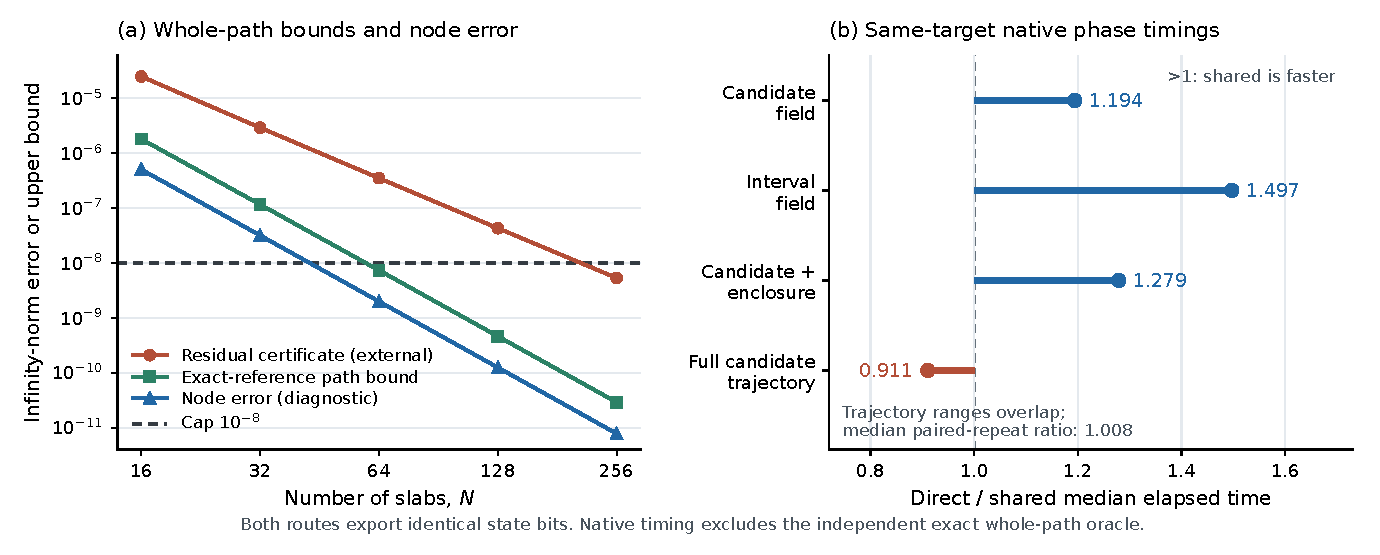
\includegraphics[width=\linewidth]{trace_results.pdf}
\caption{Trace evidence. The continuous residual certificate is more
conservative than the exact manufactured-reference bound. Field-level median
ratios exceed one, while the candidate-trajectory marginal ratio does not.
The latter has overlapping repeated ranges and is not a stable speed claim.}
\label{fig:trace}
\end{figure}

\subsection{Where certification cost is paid}

The external exact oracle internally records 10.775910623 seconds for closure,
2.564409354 seconds for trace and 13.362724506 seconds in total; process wall
time is 13.466613229 seconds. No per-route/per-grid trace oracle timings were
recorded. Apportioning this aggregate or substituting native point enclosure
time would fabricate a complete certified-trajectory ratio.

Closure already returns a native whole-path physical certificate, so that
cost belongs to its measured native total; the external oracle validates it
independently. Trace has native point/parameter-box enclosures but its
whole-path certificate in this experiment is external exact-rational code.
No native root-enumeration baseline was executed, and no speed claim against
root enumeration is made. Compilation, JSON output, independent validation
and consumer output lifetime remain explicitly outside native timing scopes.

\section{Polyalgorithm integration and remaining theoretical work}

For a common accepted target, complete cost includes session/adapter work,
candidate generation, certification and state commitment. Endpoint preparation,
failed probes, calibration, rollback and parallel workspace must be charged
once. A cheap candidate may lose after its certificate is included.
The present data concern structured provider/certificate costs and do not
measure the default switcher or mode-to-mode residence decisions.

\subsection{An exact parallel formulation with a serial baseline}

The cyclic relation has affine maps $T_i(z)=a_i+c_i z$ with $a_i=f_i$,
$c_i=-b_i$. Composition on pairs is
\begin{equation}
(a,c)\circ(d,e)=(a+cd,ce).
\end{equation}
Expanding both parenthesizations proves associativity. A cyclic composition
is $A+Cz$, so its fixed point is $A/(1-C)$; $|C|\le8^{-n}<1$ on the box.
A balanced prefix/suffix scan has $O(n)$ exact-arithmetic work and
$O(\log n)$ span. This does not parallelize arbitrary nonlinear RK stages.
The native implementation remains the low-storage $O(n)$ serial recurrence
for $n=4,8,16$. A future scan must certify reassociation roundoff or its
original tangent residual and include synchronization/workspace costs before
claiming a crossover. No new parallel hardware speedup was measured here.

\subsection{Polynomial alternatives and the actual-model remainder}

Earlier Chebyshev, Laguerre, Leja, finite-causal and quotient constructions
remain conditional routes. A symmetric real spectral interval can justify
Chebyshev minimax reasoning; eigenvalues alone do not bound a nonnormal
matrix function. Laguerre/Leja actions need a valid domain, tail/degree and
rounding bound plus an original-action certificate. A finite structural
identity removes iteration only in its declared algebra. A small projected
residual does not establish a whole ODE physical-error bound.
Selective supplied JVP/AD remains an explicit option when a comparable
derivative-free route is insufficient or costs more; no derivative callback
is silently activated by the present modules.

The pinned PR95 chemical theory has the frozen structure
\begin{align}
F(z)&=b+Pz+(e^Tz)Qz,\\
J(z)&=P+(e^Tz)Q+(Qz)e^T,\\
F(z+d)-F(z)-J(z)d&=(e^Td)Qd.
\end{align}
It can supply a verified $\Gamma\rho^2$ remainder to a near-affine causal
certificate. A different carrier $J_0$ also needs
$\|J(z)-J_0\|\rho$. Omitting electron feedback changes the original model.
Rate/time enclosures, omitted geometry, full-state norm and lift, and callback
rounding remain unclosed obligations. A conditional six-variable identity and
entrywise extremizers are not a full-model native qualification.

\subsection{A concrete next certificate question}

The gap in Table~\ref{tab:trace-accuracy} motivates further theory, not a
smaller empirical safety factor. A supremum-based defect bound can discard
signed cancellation; this is a possible mechanism, not an isolated measured
cause of the observed gap. A proposed route is the residual primitive
$\rho(t)=\int_{t_i}^t R(s)\,ds$ and corrected path $z=\widehat y-\rho$.
Then
\begin{equation}
z'-F(t,z)=F(t,\widehat y)-F(t,z).
\end{equation}
On the declared box the absolute infinity Lipschitz bound is $L=75/64$,
and the contraction rate remains $39/64$. Conditional on both paths and the
relevant tube remaining in that domain, the comparison bound returns to the
original reconstruction with an explicit $\|\rho(t)\|$ term and an integral
of $L\|\rho\|$. Exact primitive representation, finite arithmetic, domain
containment and complete cost must all be established. This is a future task;
no implementation or experimental success for it is included in this cohort.

\section{Production qualification and local handoff}

\begin{table}[h]
\caption{Separate theory and engineering obligations. Current component
success does not discharge these gates.}
\begin{ruledtabular}
\begin{tabular}{L{0.22\linewidth}L{0.35\linewidth}L{0.34\linewidth}}
Task & Mathematical obligation & Implementation/validation obligation \\
\hline
Selected singular branch & Physical selection, uniqueness and continuation at a singular point & A typed provider and original-model negative controls \\
Global F5 / generic quotient & Complete atlas, exclusions, stabilizers, local lengths, finite-free basis and denominator units & Actual multivariate provider and multiplicity checks \\
Trace path certificate & Sharper valid continuous defect/tube bound & Native outward implementation and route-specific total cost \\
Actual chemical client & Full rates/time/geometry/norm/rounding remainder & Source-bound provider and external-client validation \\
Parallel/polynomial routes & Work/span, admissible action domain and finite-error bounds & Hardware crossover with all overhead and failed probes \\
Adapter and release & Common target and continuation/rollback ownership & Ten interactions, Q-API, authority, supported features and package qualification
\end{tabular}
\end{ruledtabular}
\end{table}

The machine plan retains the original 23 nodes and 34 dependency edges, with
two bounded leaves and current source-bound results. It does not reset
correction budgets or mark the six parent N tasks complete. It is a DAG
document, not the old execution-suites parser input. The standalone Korean
Codex handoff specifies the actual eight-suite plan, exact commands, the
required Givens oracle environment and lock ownership.

The local sequence is: (LOCAL-01) establish the newly published local source
and reconstruct the preserved evidence; (LOCAL-02) integrate still-needed
ancestors once in a fresh worktree based on the latest main and complete the
cumulative API/interaction gates; (LOCAL-03) complete real-client providers;
(LOCAL-04) perform matched-cap hardware and complete-cost profiling; and
(LOCAL-05) qualify the supported release after the theory/provider and
hardware branches join. Existing valid evidence is reused within its source
and scope. Main is not merged directly, and duplicate ancestor cherry-picks
and force pushes are excluded.

The runner must receive the actual published local HEAD and its real remote
branch; the historical execution pin must not be forged by changing a
tracking ref. New scientific code requires a new source publication and
receipt. The general solver remains HOLD until authority, API, negative,
ignored-supported-feature and external-client requirements are resolved.

\section*{Artifact and reproduction guide}

The principal files under \path{research/production_rvj_nag_20261028/}
are \path{RESULTS.json}, \path{REPORT_KO.md},
\path{LOCAL_CODEX_HANDOFF_KO.md},
\path{LOCAL_DEVELOPMENT_PLAN.json},
\path{analysis/BENCHMARK_ANALYSIS.json}, and
\path{evidence/registered01/RUN_RECEIPT.json}.
The raw index supplies both compressed-file hashes and original decompressed
byte hashes. Complete repeats, refusals, source identities, actual argv,
compiler, binary hashes and timestamps are retained. The figure script only
reads frozen analysis; rebuilding this report does not rerun the solver.
The repository ledger binds compact numeric results and raw evidence.

\begin{thebibliography}{9}
\bibitem{MRD2018}
V. Magron, A. Rocca, and T. Dang,
\emph{Certified Roundoff Error Bounds using Bernstein Expansions and Sparse
Krivine--Stengle Representations}, arXiv:1802.04385v1 (2018),
\url{https://arxiv.org/html/1802.04385v1}.
\bibitem{BFSS2002}
A. Bostan, P. Flajolet, B. Salvy, and E. Schost,
\emph{Fast Computation With Two Algebraic Numbers} (2002),
\url{https://algo.inria.fr/flajolet/Publications/BoFlSaSc02.pdf}.
\bibitem{CLM2025}
J. H. Chaudhry, O. L. Lewis, and M. A. A. Molla,
\emph{Adjoint-based A Posteriori Error Analysis for Semi-explicit Index-1
and Hessenberg Index-2 Differential-Algebraic Equations},
arXiv:2507.03712v2 (2025), \url{https://arxiv.org/html/2507.03712v2}.
\end{thebibliography}
\end{document}
